\section{Strengths and weaknesses}
	Resumiendo, este documento muestra un algoritmo de tracking basado en visi\'on para ser usados en UAVs. Este algoritmo es capaz de realizar tracking de m\'ultiples objetos basados en su color. Esta caracter\'istica es una de las principales ventajas del algoritmo frente a otros como CAMSHIFT's \cite{CAMSHIFT_FAST} \cite{CAMSHIFT_ENVIROMENT}. El cuello de botella de los algoritmos de segmentaci\'on es el tiempo de computaci\'on, sin embargo el algoritmo descrito anteriormente permite al ordenador de abordo de los UAVs procesar r\'apidamente las im\'agenes capturadas.
	En paralelo al desarrollo del algoritmo se desarrol\'o una libreria multi-plataforma parar poder hacer un uso r\'apido del c\'odigo. A parte de otras ventajas que conlleva el control de versiones. El ap\'endice A \ref{chap:c6_bovil} contiene una breve descripci\'on de la librer\'ia
	% % TODO 666 ADD CITES!!
	
\section{Future Branches}	
	\subsection{Parallel Color Clustering}
	Como ya se ha comendato, el principal cuello de botella es la segmentaci\'on por color. Cada paso del algoritmo comprueba cada pixel de la im\'agen, por lo que se puede reestructurar esta parte del algoritmo con el paradigma de procesamiento paralelo. Usando la unidad de procesamiento gr\'afica (GPU) en vez de la CPU es posible aumentar notablemente la velocidad del proceso \cite{GPU_CPU_performance} \cite{GPU_parallel_image_processing} \cite{GPU_enabled_parrallel}.
		
	\begin{figure}[ph]
		\centering
		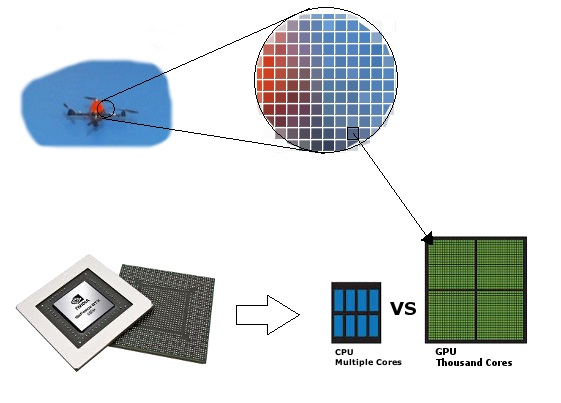
\includegraphics[width=0.7\linewidth]{../Images/c5/gpu}
		\caption{Paralelizaci\'on}
		\label{fig:gpu}
	\end{figure}


	\subsection{Reconocimiento de Formas}
	Hasta ahora, el criterio de selecci\'on de objetivo se realiza por color y tama\~no. Sin embargo esto puede causar problemas cuando existen m\'ultiples posibles objetivos en la escena. El reconocimiento de patrones o formas  \cite{color_shape_object_recogn} \cite{Fast_object_recogn_shape} podr\'ia ser una herramienta muy \'util para esta parte del algoritmo:
	
	\begin{figure}[th]
		\centering
		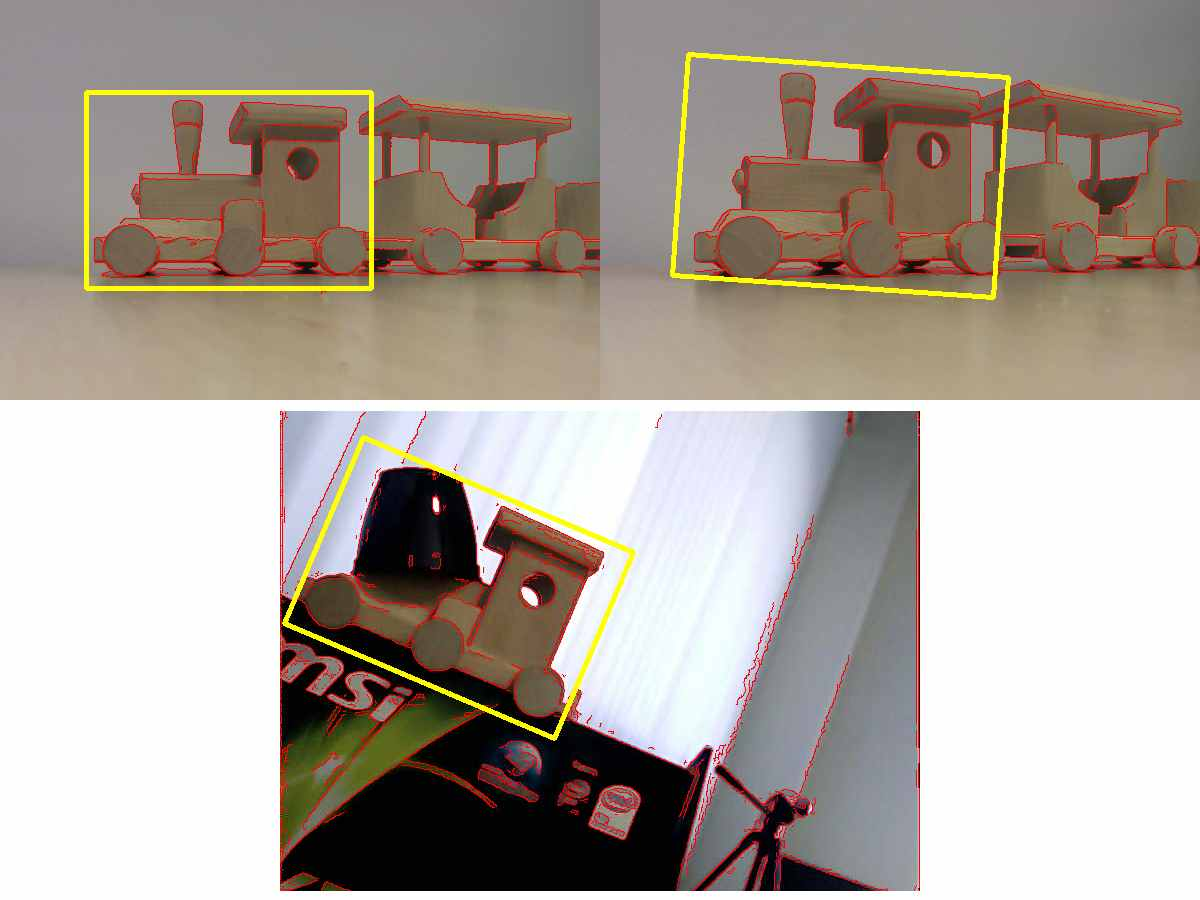
\includegraphics[width=0.6\linewidth]{../Images/c6/shape_recogn}
		\caption{Reconocimiento de Formas}
		\label{fig:shape_recogn}
	\end{figure}
	
	\subsection{Big Data}
	Este t\'ermino se refiere  a la recolecci\'on de grandes cantidades de datos con estructuras diversas y complejas. En este punto resulta complicado procesar esa cantidad de informaci\'on. Plantear una correcta arquitectura para el "Data mining" \cite{Big_data_Ecosystem} \cite{Big_data_mapReduce} puede prevenir al sistema de colapsar en caso de grandes caudales de informaci\'on:
	
	\begin{figure}[th]
		\centering
		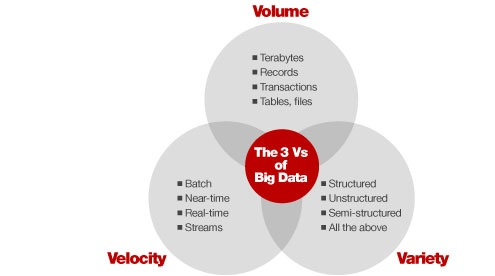
\includegraphics[width=0.7\linewidth]{../Images/c6/big_data}
		\caption{Big Data}
		\label{fig:big_data}
	\end{figure}
	
	
